\UC{Aggiunta nuova categoria}
\label{aggiunta-categoria}

\begin{figure}[H]
    \centering
    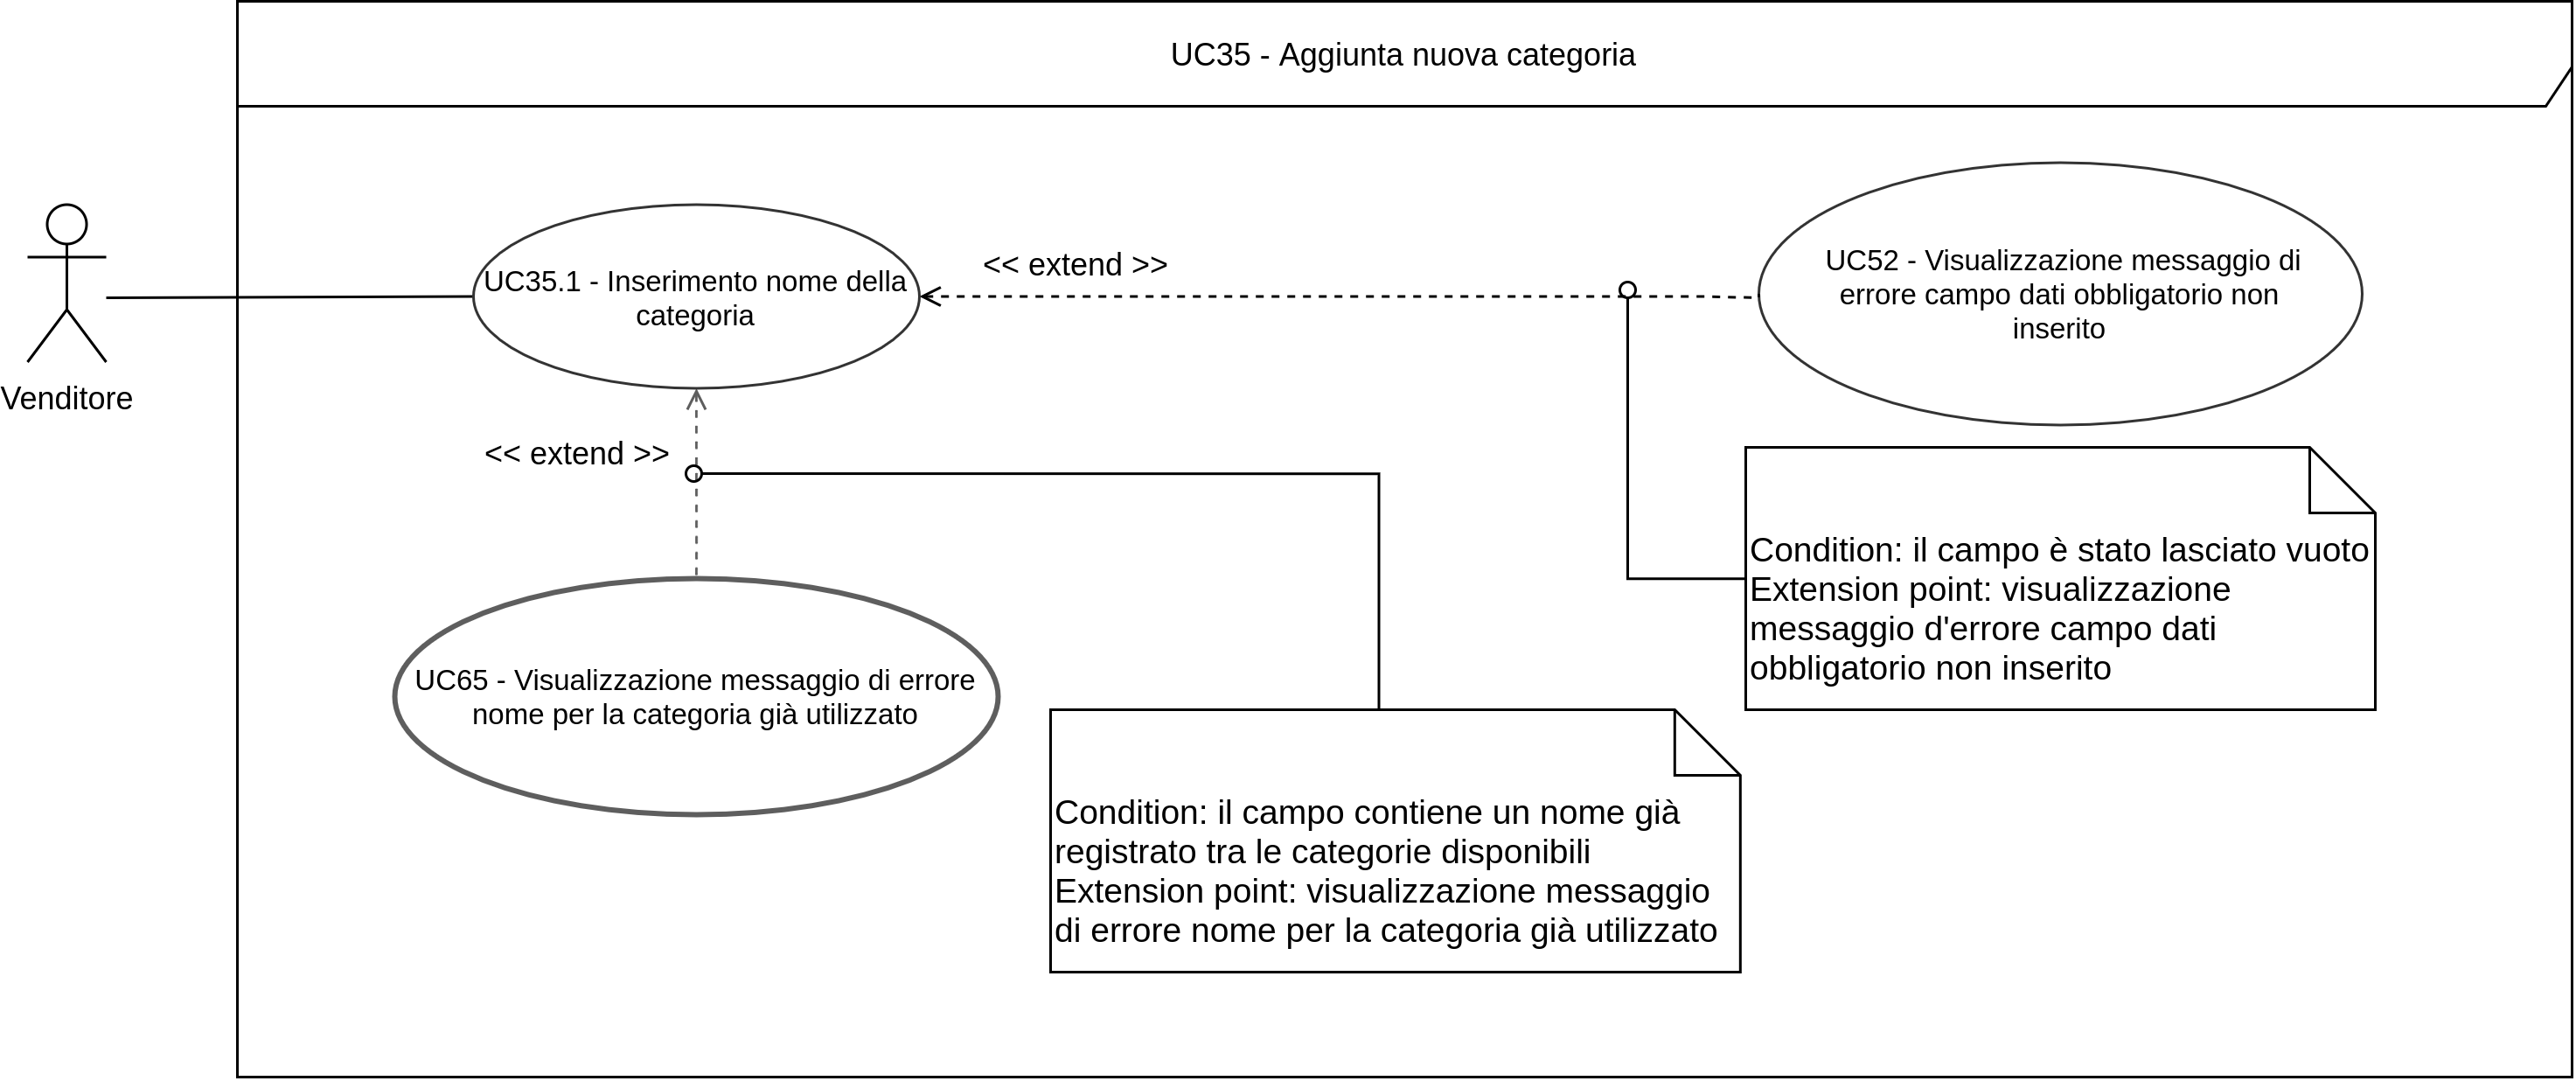
\includegraphics[width=\textwidth]{Immagini/DiagrammiUC/Venditore/AggiuntaCategoria.png}
    \caption{Diagramma di \actualUC: Aggiunta nuova categoria}
    \label{fig:aggiunta-categoria}
\end{figure}

Il venditore aggiunge una nuova categoria.
\begin{itemize}
    \item \textbf{Attori primari:} venditore;
    \item \textbf{Precondizione:} il venditore si trova nella schermata di amministrazione delle categorie e ha selezionato la funzionalità di aggiunta di una nuova categoria;
    \item \textbf{Postcondizione:} la categoria inserita è stata creata;
    \item \textbf{Scenario principale:}
    \begin{itemize}
    	\item Il venditore si trova nella schermata di amministrazione delle categorie;
    	\item Il venditore seleziona la funzionalità per aggiungere una nuova categoria di prodotti;
    	\item (UC\ref{aggiunta-categoria.nome}) - Inserimento nome della nuova categoria;
    	\item Il venditore conferma la creazione della categoria di prodotti.
    \end{itemize} 
    \item \textbf{Scenari alternativi:}
    \begin{enumerate}[label=\lett]
    	\item Il venditore non conferma la creazione della categoria e di conseguenza questa non verrà aggiunta.
    \end{enumerate}
\end{itemize}

\subUC{Inserimento nome della categoria}
\label{aggiunta-categoria.nome}

Il venditore inserisce il nome della nuova categoria da aggiungere.
\begin{itemize}
    \item \textbf{Attori primari:} venditore;
    \item \textbf{Precondizione:} il venditore sta eseguendo l'azione di aggiunta di una nuova categoria;
    \item \textbf{Postcondizione:} il venditore ha inserito il nome della categoria;
    \item \textbf{Scenario principale:} il venditore compila il modulo per l'aggiunta della nuova categoria inserendo un nome;
    \item \textbf{Estensioni:}
    \begin{enumerate}[label=\lett]
    	\item Il venditore non inserisce alcun nome per la nuova categoria. In questo caso:
    	\begin{itemize}
    		\item (UC\ref{estensione:campo-obbligatorio-non-inserito}) - Verrà visualizzato il messaggio di errore campo dati obbligatorio non inserito;
    		\item Viene fornita al venditore la possibilità di modificare il nome della nuova categoria di prodotti.
    	\end{itemize}
    	\item Il venditore inserisce un nome per la nuova categoria che è già assegnato ad un'altra categoria. In questo caso:
    	\begin{itemize}
    		\item (UC\ref{estensione:categoria-esistente}) - Verrà visualizzato il messaggio di errore nome per la categoria già utilizzato;
    		\item Viene fornita al venditore la possibilità di modificare il nome della nuova categoria di prodotti.
    	\end{itemize}
    \end{enumerate}
\end{itemize}

\UC{Modifica di una categoria}
\label{modifica-categoria}

\begin{figure}[H]
    \centering
    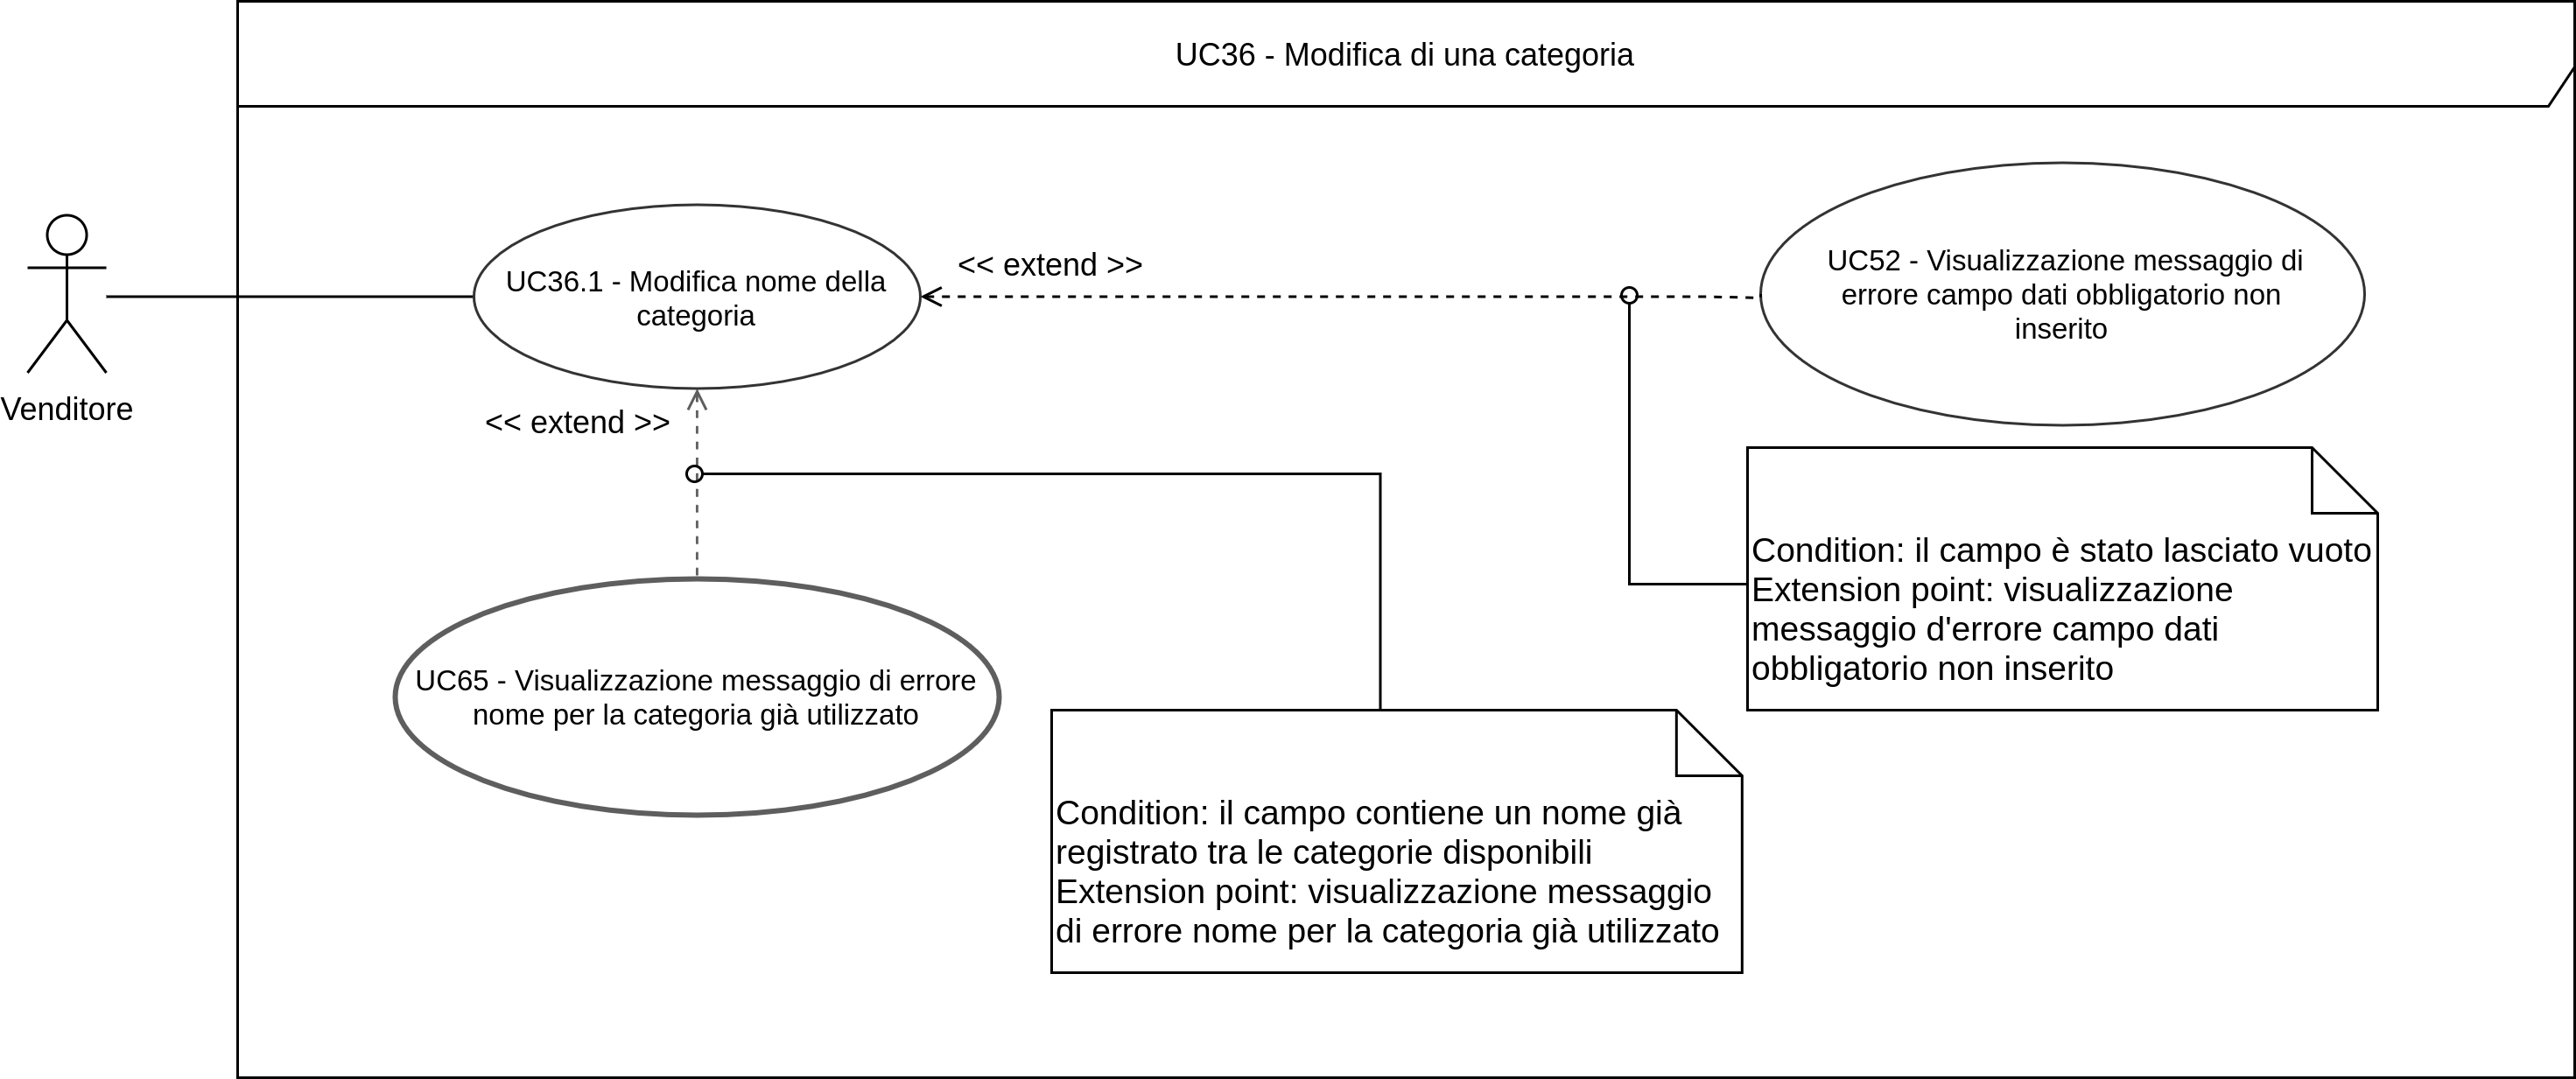
\includegraphics[width=\textwidth]{Immagini/DiagrammiUC/Venditore/ModificaCategoria.png}
    \caption{Diagramma di \actualUC: Modifica di una categoria}
    \label{fig:modifica-categoria}
\end{figure}

Il venditore modifica una categoria precedentemente inserita.
\begin{itemize}
    \item \textbf{Attori primari:} venditore;
    \item \textbf{Precondizione:} il venditore si trova nella schermata di amministrazione delle categorie e ha selezionato la funzionalità di modifica di una categoria precedentemente inserita;
    \item \textbf{Postcondizione:} la categoria selezionata viene modificata;
    \item \textbf{Scenario principale:}
    \begin{itemize}
    	\item Il venditore si trova nella schermata di amministrazione delle categorie;
    	\item Il venditore seleziona la funzionalità per modificare una categoria di prodotti;
    	\item (UC\ref{modifica-categoria.nome}) - Modifica nome della categoria;
    	\item Il venditore conferma la modifica della categoria di prodotti.
    \end{itemize}
    \item \textbf{Scenari alternativi:} 
    \begin{enumerate}[label=\lett]
    	\item Il venditore non dà la conferma alle modifiche effettuate e di conseguenza la categoria non verrà modificata.
    \end{enumerate}
\end{itemize}

\subUC{Modifica nome della categoria}
\label{modifica-categoria.nome}

Il venditore modifica il nome attuale di una categoria precedentemente inserita.
\begin{itemize}
    \item \textbf{Attori primari:} venditore;
    \item \textbf{Precondizione:} il venditore sta eseguendo l'azione di modifica di una categoria;
    \item \textbf{Postcondizione:} il venditore ha modificato il nome della categoria;
    \item \textbf{Scenario principale:} il venditore modifica la categoria inserendo un nuovo nome o modificando quello attuale;
    \item \textbf{Estensioni:}
    \begin{enumerate}[label=\lett]
    	\item Il venditore elimina il nome utilizzato in precedenza non inserendone uno nuovo. In questo caso:
    	\begin{itemize}
    		\item (UC\ref{estensione:campo-obbligatorio-non-inserito}) - Verrà visualizzato il messaggio di errore campo dati obbligatorio non inserito;
    		\item Viene fornita al venditore la possibilità di modificare il nome della nuova categoria di prodotti.
    	\end{itemize}
    	\item Il venditore modifica il nome della categoria con uno che è già assegnato ad un'altra categoria. In questo caso:
		\begin{itemize}
			\item (UC\ref{estensione:categoria-esistente}) - Verrà visualizzato il messaggio di errore nome per la categoria già utilizzato;
			\item Viene fornita al venditore la possibilità di modificare il nome della nuova categoria di prodotti.
		\end{itemize}
    \end{enumerate}
\end{itemize}

\UC{Eliminazione di una categoria}
\label{eliminazione-categoria}

Il venditore elimina una categoria precedentemente inserita.
\begin{itemize}
    \item \textbf{Attori primari:} venditore;
    \item \textbf{Precondizione:} il venditore si trova nella schermata di amministrazione delle categorie e ha selezionato la funzionalità di eliminazione di una categoria precedentemente inserita;
    \item \textbf{Postcondizione:} la categoria interessata viene eliminata;
    \item \textbf{Scenario principale:}
    \begin{itemize}
    	\item Il venditore si trova nella schermata di amministrazione delle categorie;
    	\item Il venditore seleziona la funzionalità per eliminare una categoria di prodotti;
    	\item Il venditore conferma la rimozione della categoria di prodotti con la conseguente eliminazione anche nei prodotti appartenenti alla categoria indicata.
    \end{itemize}
    \item \textbf{Scenari alternativi:}
    \begin{enumerate}[label=\lett]
    	\item Durante la visualizzazione del messaggio di conferma, il venditore non da il suo consenso per l'eliminazione e di conseguenza la categoria non verrà eliminata.
    \end{enumerate}
\end{itemize}

\UC{Ricerca categoria}
\label{ricerca-categoria}

Il venditore può cercare una categoria dalla propria schermata di amministrazione delle categorie.
\begin{itemize}
	\item \textbf{Attori primari:} venditore;
	\item \textbf{Precondizione:} il venditore ha selezionato la funzionalità per la ricerca;
	\item \textbf{Postcondizione:} il venditore visualizza le categorie che contengono nel nome almeno una delle parole per le quali si è svolta la ricerca;
	\item \textbf{Scenario principale:} il venditore ha selezionato la funzione prevista per la ricerca. Dopo aver inserito le parole per le quali individuare la categoria, avvia la ricerca e viene aggiornata la schermata di amministrazione delle categorie la quale visualizzerà tutte le categorie che hanno almeno una delle parole indicate nel nome;
	\item \textbf{Scenari alternativi:}
	\begin{enumerate}[label=\lett]
		\item Il venditore ha svolto una ricerca che non ha trovato coincidenze con nessuna categoria. In questo caso la schermata di amministrazione delle categorie viene aggiornata mostrando il messaggio nessuna categoria trovata.
	\end{enumerate}
\end{itemize}